\section{PCA Feature Maps.}
\label{app:feature_maps}

\paragraph{Construction of PCA Feature Maps.}

A SiT-B/2 transformer processes its input as a sequence of spatial patches.
After the VAE encodes a $256{\times}256$ image into a $32{\times}32{\times}4$
latent $z_0$, a patch embedding layer with patch size~2 splits this into
$16{\times}16 = 256$ tokens, each carrying a 768-dimensional feature vector.
At every transformer block $\ell \in \{1, \dots, 12\}$ the model produces a
hidden state matrix
\[
  H^{(\ell)} \in \mathbb{R}^{256 \times 768}.
\]
To visualise the geometry of this representation space, forward hooks are
registered on every block simultaneously so that a \emph{single} forward pass
captures all 12 hidden states at once. The input to the model is a noisy
latent constructed via the linear stochastic interpolant
\[
  z_t = (1 - t)\,z_0 + t\,\varepsilon, \quad
  \varepsilon \sim \mathcal{N}(0, I),
\]
evaluated at three noise levels $t \in \{0.5,\, 0.7,\, 0.9\}$ to probe how
representations change as the signal-to-noise ratio decreases.

At each block the 256 token vectors are projected to three dimensions via PCA:
\[
  \widetilde{H}^{(\ell)} = \operatorname{PCA}_3\!\left(H^{(\ell)}\right)
  \in \mathbb{R}^{256 \times 3}.
\]
Each component is normalised channel-wise to $[0, 1]$, reshaped to a
$16{\times}16{\times}3$ spatial grid, and upsampled to $128{\times}128$ pixels
for display. Patches whose token vectors are similar appear in the same colour,
so the map is a spatial portrait of what the model considers semantically
equivalent at that depth.

A critical implementation detail is that the PCA for each layer is fitted
\emph{jointly} on the concatenated token matrices of the Baseline and REPA
models:
\[
  \operatorname{PCA}_3\!\Bigl(
    \bigl[H^{(\ell)}_{\text{Base}};\; H^{(\ell)}_{\text{REPA}}\bigr]
  \Bigr),
\]
so both models share the same colour axes. Without this, a colour difference
between the two maps could reflect an arbitrary rotation of the PCA solution
rather than a genuine representational difference. The joint fitting guarantees
that identical colours encode identical representations across models.



\paragraph{Layer-wise Progression and Noise Robustness.}

Figure~\ref{fig:pca_layers} shows PCA feature maps for a representative image
across all 12 transformer blocks and three noise levels $t \in \{0.5, 0.7,
0.9\}$. For each timestep, rows correspond to the original photograph, the
Baseline PCA map, and the REPA PCA map respectively, with transformer blocks
as columns.

\begin{figure}[t]
  \centering
  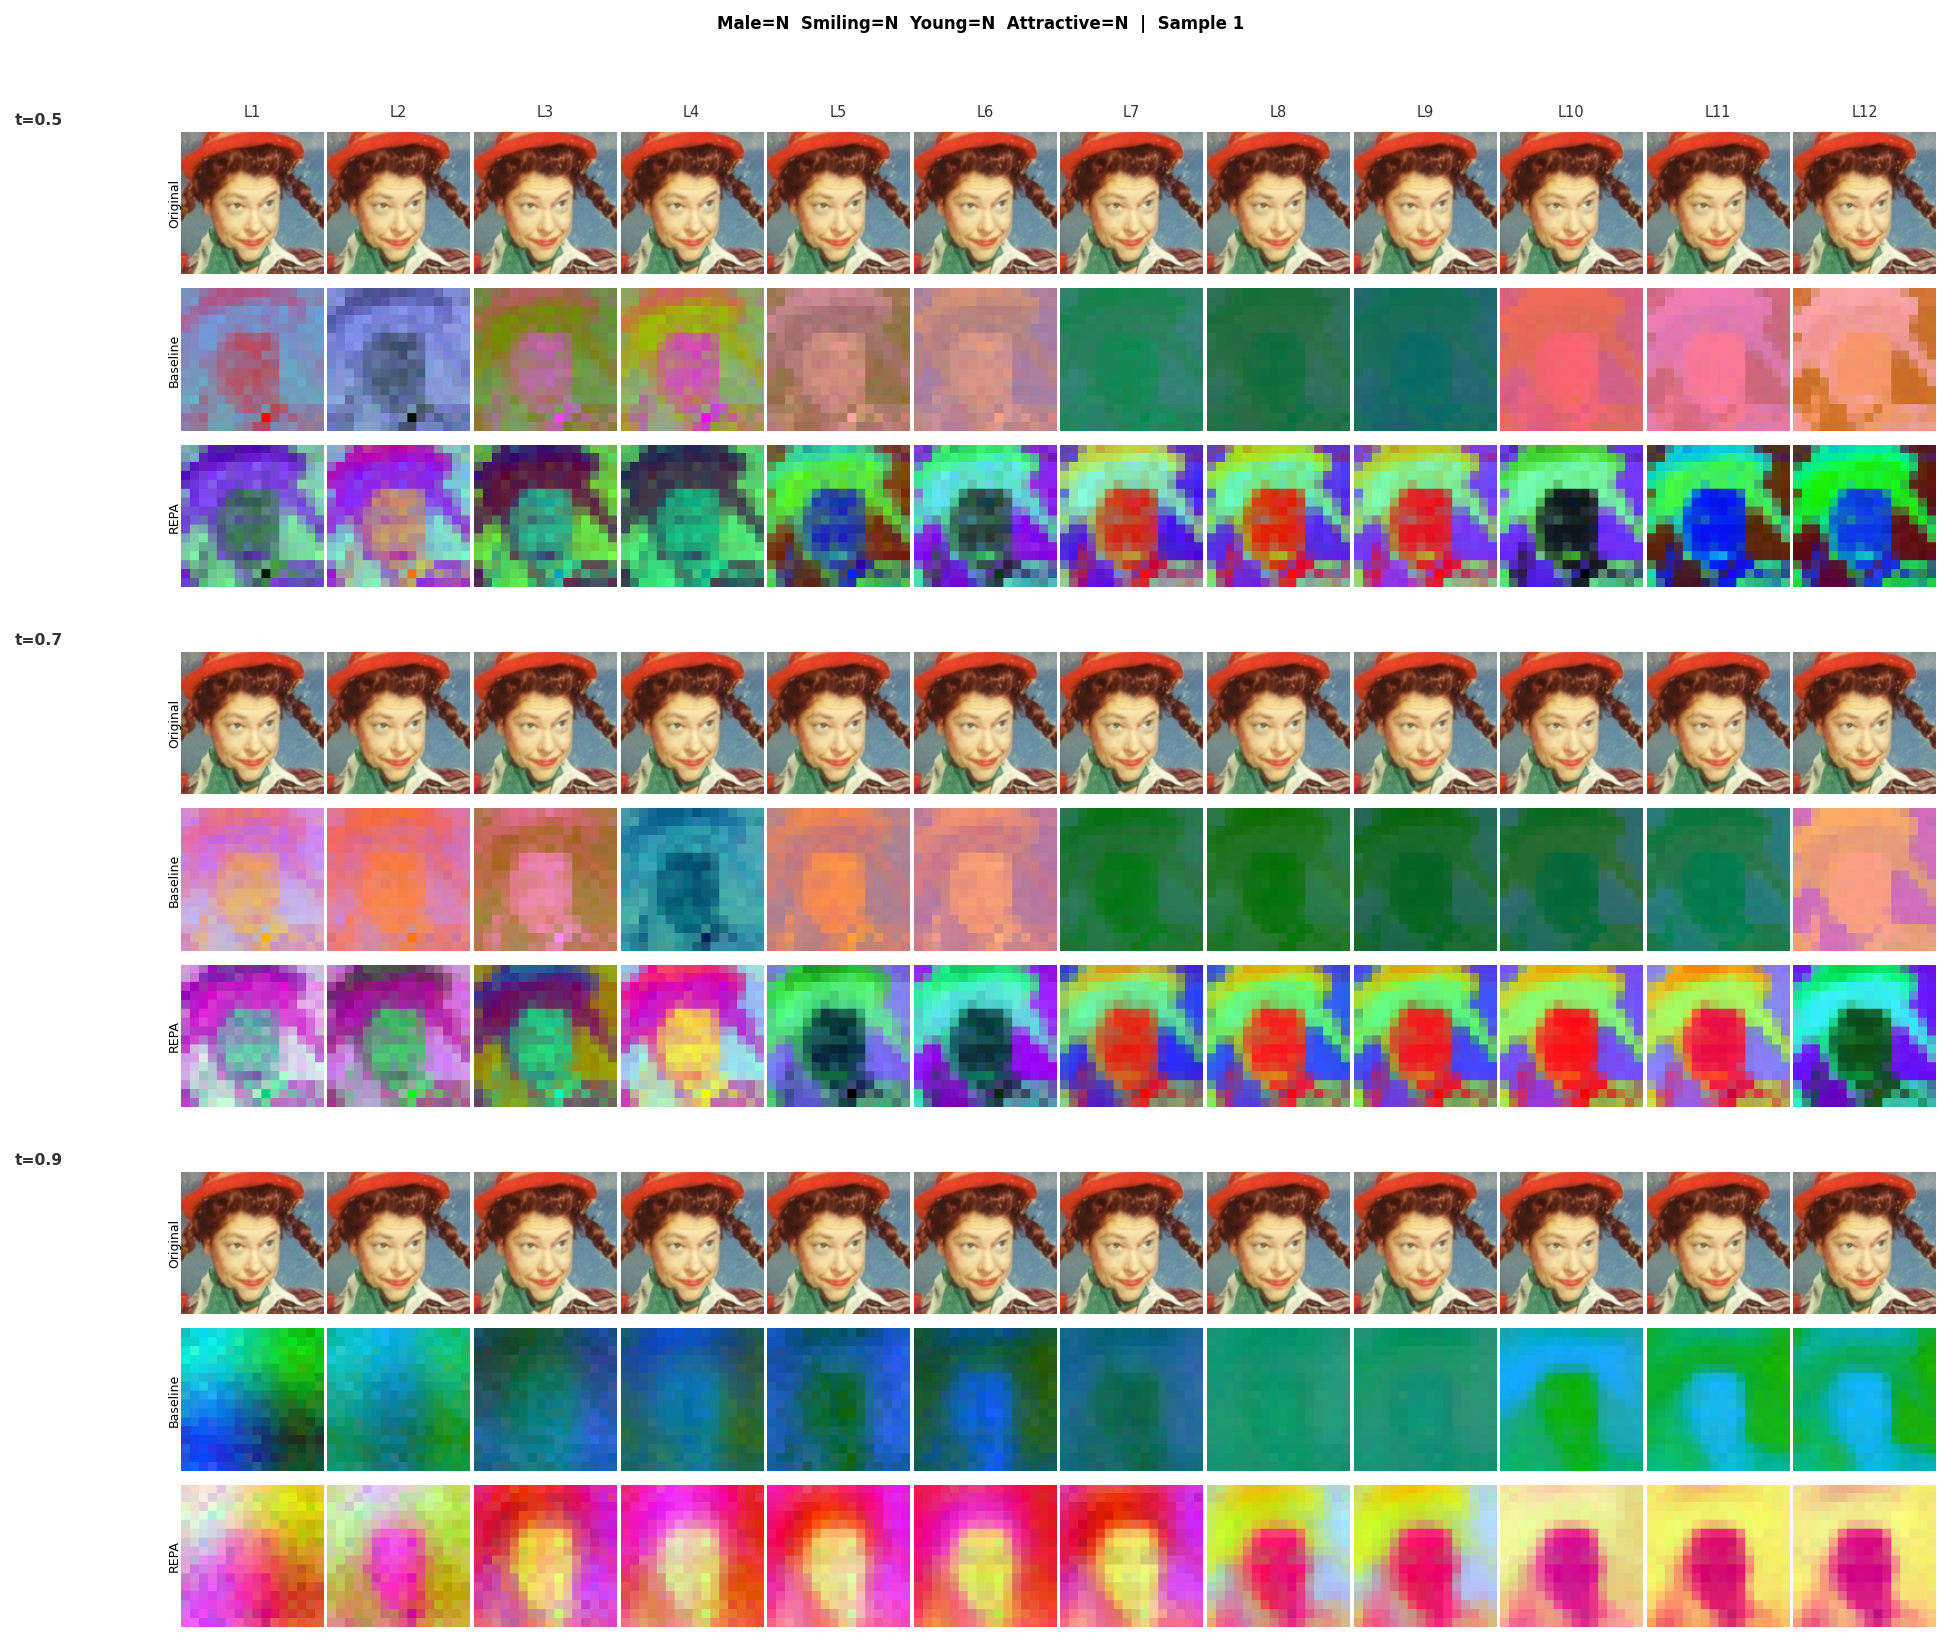
\includegraphics[width=\linewidth]{images/noise_layers.png}
  \caption{%
    PCA feature maps across all 12 transformer blocks and three noise levels.
    For each timestep group, rows show: the original CelebA image, the
    Baseline hidden-state PCA map, and the REPA hidden-state PCA map.
    Columns correspond to transformer blocks 1--12 (left to right).
  }
  \label{fig:pca_layers}
\end{figure}

In both the \emph{Baseline} and \emph{REPA} models, semantic structure is already present in the early layers. From blocks 1 -- 6 at $t = 0.5$ and $t = 0.7$, the PCA maps of both models show clear spatial partitioning: face, hair, and background regions are assigned distinct colour clusters. This is consistent with the observation made earlier that CelebA's spatial homogeneity makes basic face-region separation a low-effort task that both models learn readily.

The critical difference between the two models appears in blocks~7--9, where the Baseline maps collapse into spatially incoherent noise while the REPA maps maintain structured, interpretable regions. This mid-network collapse in the Baseline suggests that its intermediate representations undergo an unstructured transition between the early feature-building phase and the final velocity-prediction layers. REPA's alignment regularisation, acting at block~8, anchors this transition: instead of dissolving into noise, the representations remain semantically organised through the middle of the network.

The timestep axis amplifies this contrast sharply. At $t = 0.9$ (near-pure Gaussian noise) the Baseline maps are largely uniform and flat from block~3 onward, recovering only a faint spatial gradient in the final blocks. REPA maps at $t = 0.9$, by contrast, retain a coherent face-background separation throughout most of the network depth, with the characteristic face-centred blob clearly visible even in layers 5--8. This confirms that REPA does not merely reorganise representations that the Baseline would form anyway -- it builds representations that are fundamentally more robust to the destruction of pixel-level signal.

To summarise, Representation Alignment produces two distinct effects visible in this figure: it \emph{stabilises} the mid-network transition that causes blocks~7--9 to collapse in the Baseline, and it makes the resulting representations \emph{noise-robust}, preserving semantic structure at timesteps where the Baseline loses it entirely.

\paragraph{Attribute-Specific Separability.}

Our training setup conditions the model on 16 class labels derived from four
binary attributes: \emph{Male}, \emph{Smiling}, \emph{Young}, and
\emph{Attractive}. This allows us to assess whether REPA's representational
improvements are attribute-dependent -- an analysis that goes beyond the
original paper's ImageNet evaluation.

Figure~\ref{fig:attr_sep} shows representative image pairs for each attribute,
selected automatically to satisfy three constraints. First, each pair is
\emph{controlled}: the two images belong to class labels that differ in exactly
one attribute bit while all other three attributes are identical, isolating the
effect of the target attribute. Second, pairs are required to be visually
similar in terms of pixel-level MSE, controlling for pose, lighting, and
background. Third, no image is reused across attribute panels. Among candidate
pairs satisfying these constraints, we select the one that maximises the
relative gain in mean patch-level cosine distance under REPA compared to the
Baseline:
\[
  \text{score} = \frac{d_{\text{REPA}} - d_{\text{Baseline}}}
                      {d_{\text{Baseline}} + \varepsilon},
  \quad
  d(A, B) = 1 - \frac{1}{N}\sum_{n=1}^{N}
    \frac{A^{[n]} \cdot B^{[n]}}{\|A^{[n]}\|\,\|B^{[n]}\|}.
\]

\begin{figure}[t]
  \centering
  
\includegraphics[width=\linewidth]{images/attribute_separation.png}
  \caption{%
    Attribute-specific feature map separability at block~8 and $t = 0.5$.
    The figure is arranged as a $2{\times}2$ grid of attribute panels
    (Male, Smiling, Young, Attractive).
    Within each panel, the two rows show images differing only in the target
    attribute (all other attributes held fixed); columns show the original
    photograph, the Baseline PCA map, and the REPA PCA map.
    Pairs were selected automatically to be visually similar and to maximise
    REPA's relative token-space separation gain over Baseline.
  }
  \label{fig:attr_sep}
\end{figure}

The results exhibit a clear attribute-dependent hierarchy.
\emph{Male} shows the largest visual separation under REPA: colour clusters
corresponding to hair, skin tone, and facial structure diverge markedly between
the Male=N and Male=Y rows in the REPA maps, while the Baseline maps remain
nearly indistinguishable. Gender is one of the strongest signals encoded by
DINOv2, providing a rich teacher signal for the alignment loss.
\emph{Smiling} produces a spatially localised effect: a distinct patch
cluster appears around the lower-face region for Smiling=Y images in the REPA
maps, reflecting alignment of mouth-area tokens with DINOv2 features sensitive
to facial expression; this cluster is absent in the Baseline.
\emph{Young} yields moderate gains, consistent with age-related textural
information (skin smoothness, fine structure) being captured by DINOv2 but less
saliently than gender or expression.
\emph{Attractive} shows the smallest improvement. The attribute is
subjectively defined and inconsistently grounded in low-level visual features,
so the DINOv2 teacher provides a weaker alignment signal and the representational
gain is correspondingly smaller.

This hierarchy reflects a fundamental property of the REPA framework: it can
only transfer structure that the self-supervised teacher itself encodes. The
LDA separability of DINOv2 features with respect to each attribute therefore
acts as an upper bound on the representational gain that REPA can deliver.

\paragraph{Attribute Direction Vector Analysis}

For each target attribute
$a \in \{\text{Male}, \text{Smiling}, \text{Young}, \text{Attractive}\}$, we
construct matched class pairs $(c_k^{+}, c_k^{-})$ that differ only in attribute
$a$ while keeping the other three conditioning attributes fixed. For every pair,
we sample the same initial Gaussian latent and generate two final VAE latents,
one conditioned on $c_k^{+}$ and one conditioned on $c_k^{-}$. This produces two
sets of generated latents, $\{z_i^{+}\}$ and $\{z_i^{-}\}$, where the comparison
is controlled for the random seed and for all non-target attributes.

We then flatten each latent and learn an attribute direction using
ridge-regularised linear regression. Let $x_i=\operatorname{vec}(z_i)$ and
$y_i \in \{+1,-1\}$ denote whether the latent was generated with the positive or
negative value of the target attribute. We fit a linear score
\[
  s_a(x) = w_a^\top (x - \bar{x})
\]
by minimizing
\[
  \sum_i \left(w_a^\top (x_i-\bar{x}) - y_i\right)^2
  + \lambda \|w_a\|_2^2 .
\]
The resulting vector $w_a$ is orthogonal to the learned separating hyperplane,
so it gives the direction in latent space that most strongly separates the two
attribute values under this linear model. We normalise this vector and rescale it
to match the typical distance between matched positive and negative latent pairs.

Finally, we test whether this direction is semantically meaningful by editing
generated latents directly. Given a base generated latent $z$, we form
\[
  z(\alpha) = z + \alpha d_a,
\]
where $d_a$ is the normalised attribute direction and $\alpha$ is a scalar sweep
coefficient. Decoding $z(\alpha)$ with the VAE gives an image sequence in which
only the target attribute should change if the direction is well isolated.
Figure~\ref{fig:young_direction_sweep} shows this procedure for the
\emph{Young} attribute. Both the baseline and REPA models produce coherent
age-related changes as $\alpha$ is varied, indicating that both generators manage
to encode this attribute as an approximately linear vector direction in latent
space.

\begin{figure}[h]
  \centering
  \begin{subfigure}[b]{\linewidth}
    \centering
    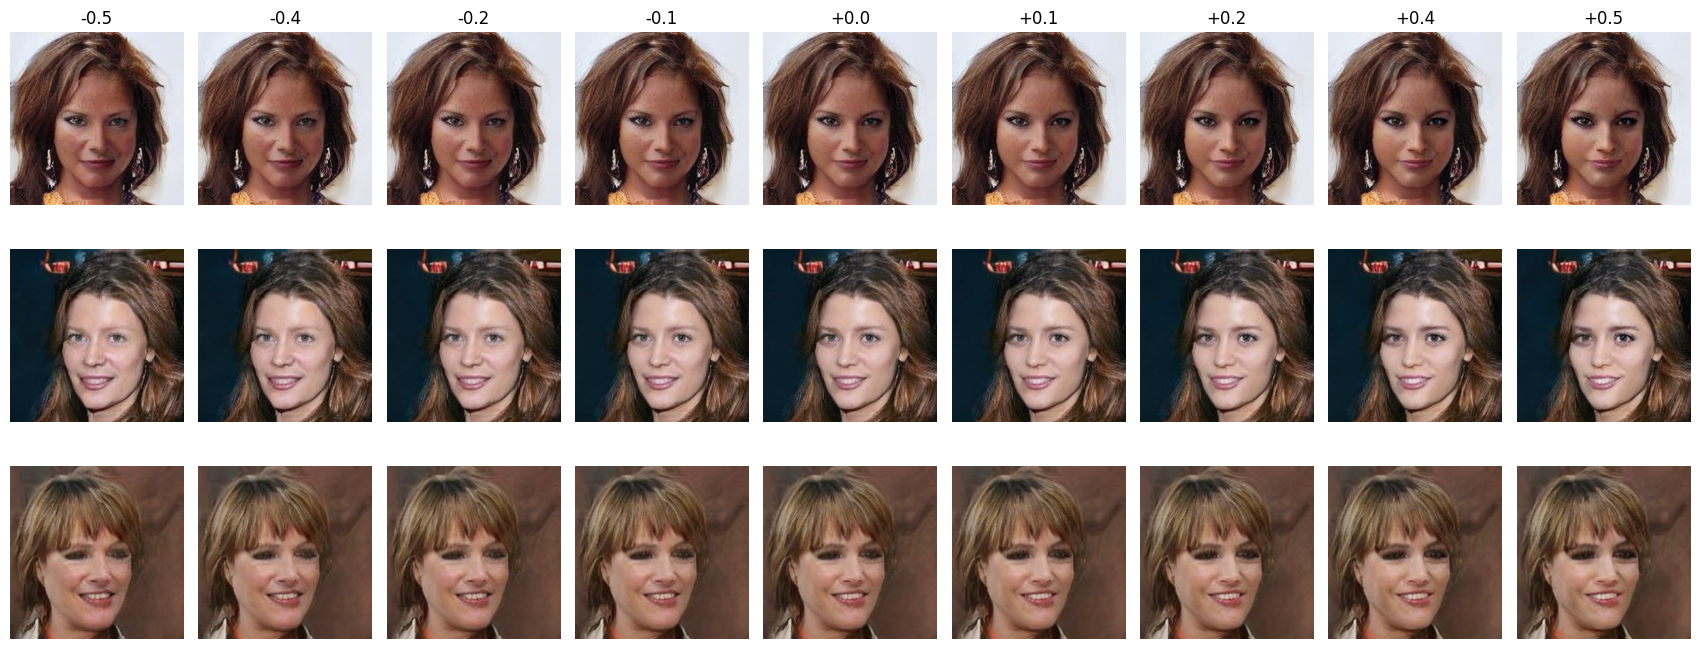
\includegraphics[width=\linewidth]{images/young_base.png}
    \caption{Baseline}
    \label{fig:young_direction_base}
  \end{subfigure}
  \vspace{0.4em}
  \begin{subfigure}[b]{\linewidth}
    \centering
    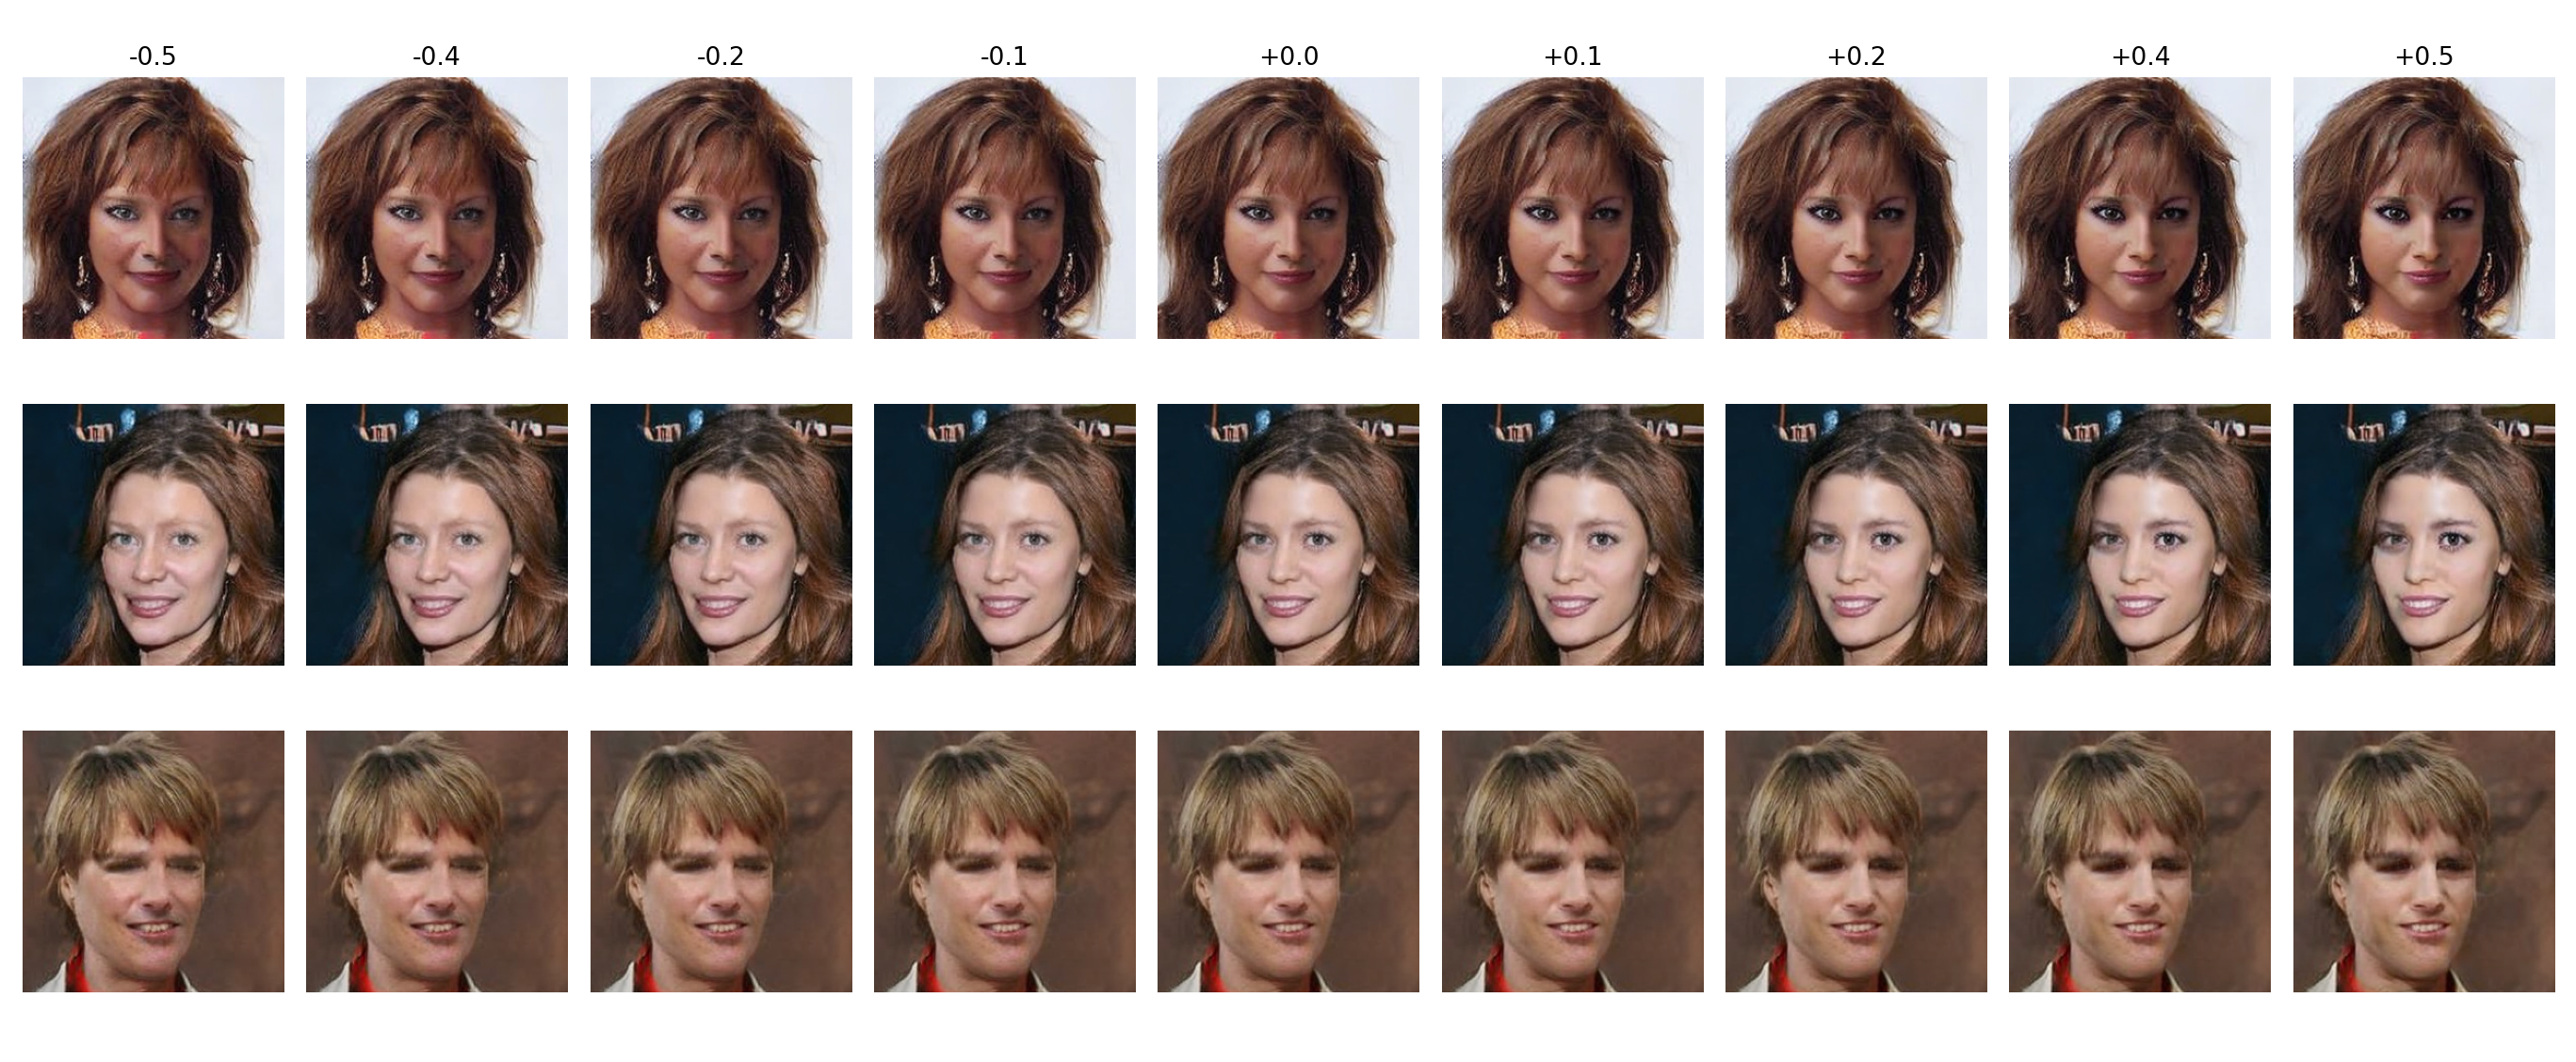
\includegraphics[width=\linewidth]{images/young_repa.png}
    \caption{REPA}
    \label{fig:young_direction_repa}
  \end{subfigure}
  \caption{Latent-space sweeps along the learned \emph{Young} attribute
  direction. Columns correspond to increasing coefficients $\alpha$ in
  $z(\alpha)=z+\alpha d_{\mathrm{Young}}$.}
  \label{fig:young_direction_sweep}
\end{figure}
